
%(BEGIN_QUESTION)
% Copyright 2010, Tony R. Kuphaldt, released under the Creative Commons Attribution License (v 1.0)
% This means you may do almost anything with this work of mine, so long as you give me proper credit

Suppose someone builds a dual-junction thermocouple circuit using type T thermocouple wire (copper and constantan metals), then measures voltage in the loop using a voltmeter:

$$\includegraphics[width=15.5cm]{i02948x01.eps}$$

Calculate the voltage read by the voltmeter, using a type T thermocouple table to find millivolt potentials for each of the junctions.

\underbar{file i02948}
%(END_QUESTION)





%(BEGIN_ANSWER)

The voltmeter should read $-3.908$ millivolts.  Counting all the junction voltages (with polarities shown in reference to whether they match or oppose the meter's test lead polarity):

\begin{itemize}
\item{} 193 $^{o}$F junction = $-3.789$ mV
\item{} 71 $^{o}$F junction = +0.857 mV
\item{} 102 $^{o}$F junction = $-1.565$ mV
\item{} 59 $^{o}$F junction = +0.589 mV
\item{} {\bf Loop total voltage} = $-3.908$ mV
\end{itemize}

Hint: any junction pushing conventional flow in a counter-clockwise direction is regarded here as a ``positive'' figure.  Any junction pushing in a clockwise direction is regarded as a ``negative'' figure.

The last junction (at 59 $^{o}$F) may be treated as a {\it single} copper-constantan junction because the metal type of the meter's test leads acts as an {\it intermediate} metal.  The fact that both the copper-testlead and constantan-testlead junctions are at the same temperature allows us to disregard the test lead metal altogether and treat it as a single copper-constantan junction at 59 $^{o}$F.

%(END_ANSWER)





%(BEGIN_NOTES)


%INDEX% Measurement, temperature: thermocouple

%(END_NOTES)


